% \section{Simulation Environment Setup}
% \label{app:simulation_setup}

% % Appendix snippet. Expected packages in the main paper:
% % \usepackage{booktabs}
% % \usepackage{array}
% % \usepackage{amsmath,amssymb}

% \section{Simulation Setting}
% \label{app:simulation-setting}

% \subsection{Common Environment Interface}
% \begin{figure}[t]
%     \centering
%     \begin{minipage}[t]{0.75\textwidth}
%         \centering
%         \vspace{0pt}
%         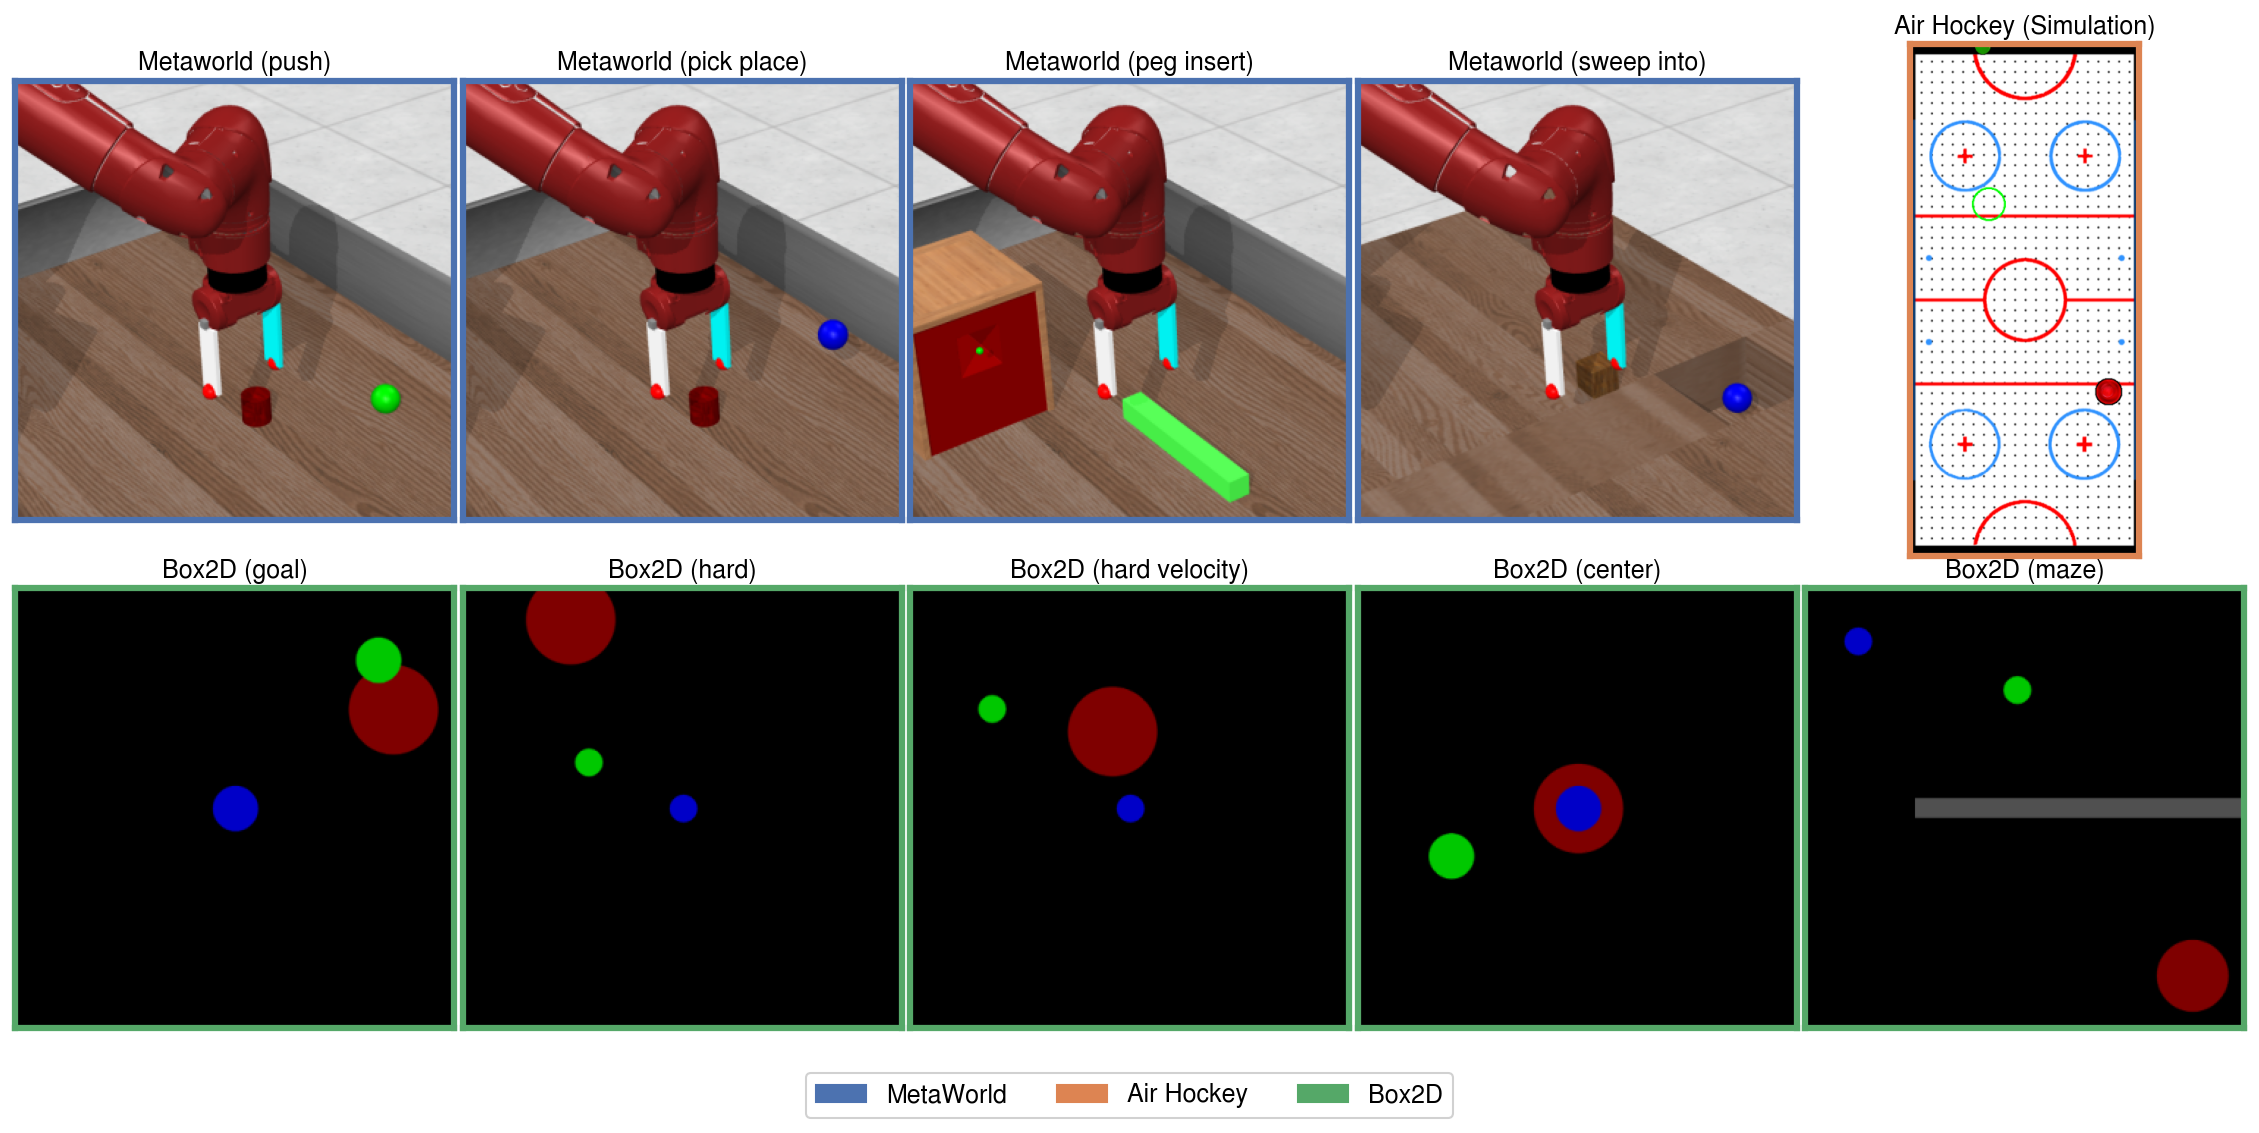
\includegraphics[width=\linewidth]{figure/task_set_figure.png}
%         \caption{Task sets used in the simulation experiments.}
%         \label{fig:task_set}
%     \end{minipage}%
%     \begin{minipage}[t]{0.25\textwidth}
%         \centering
%         \vspace{0pt}
%         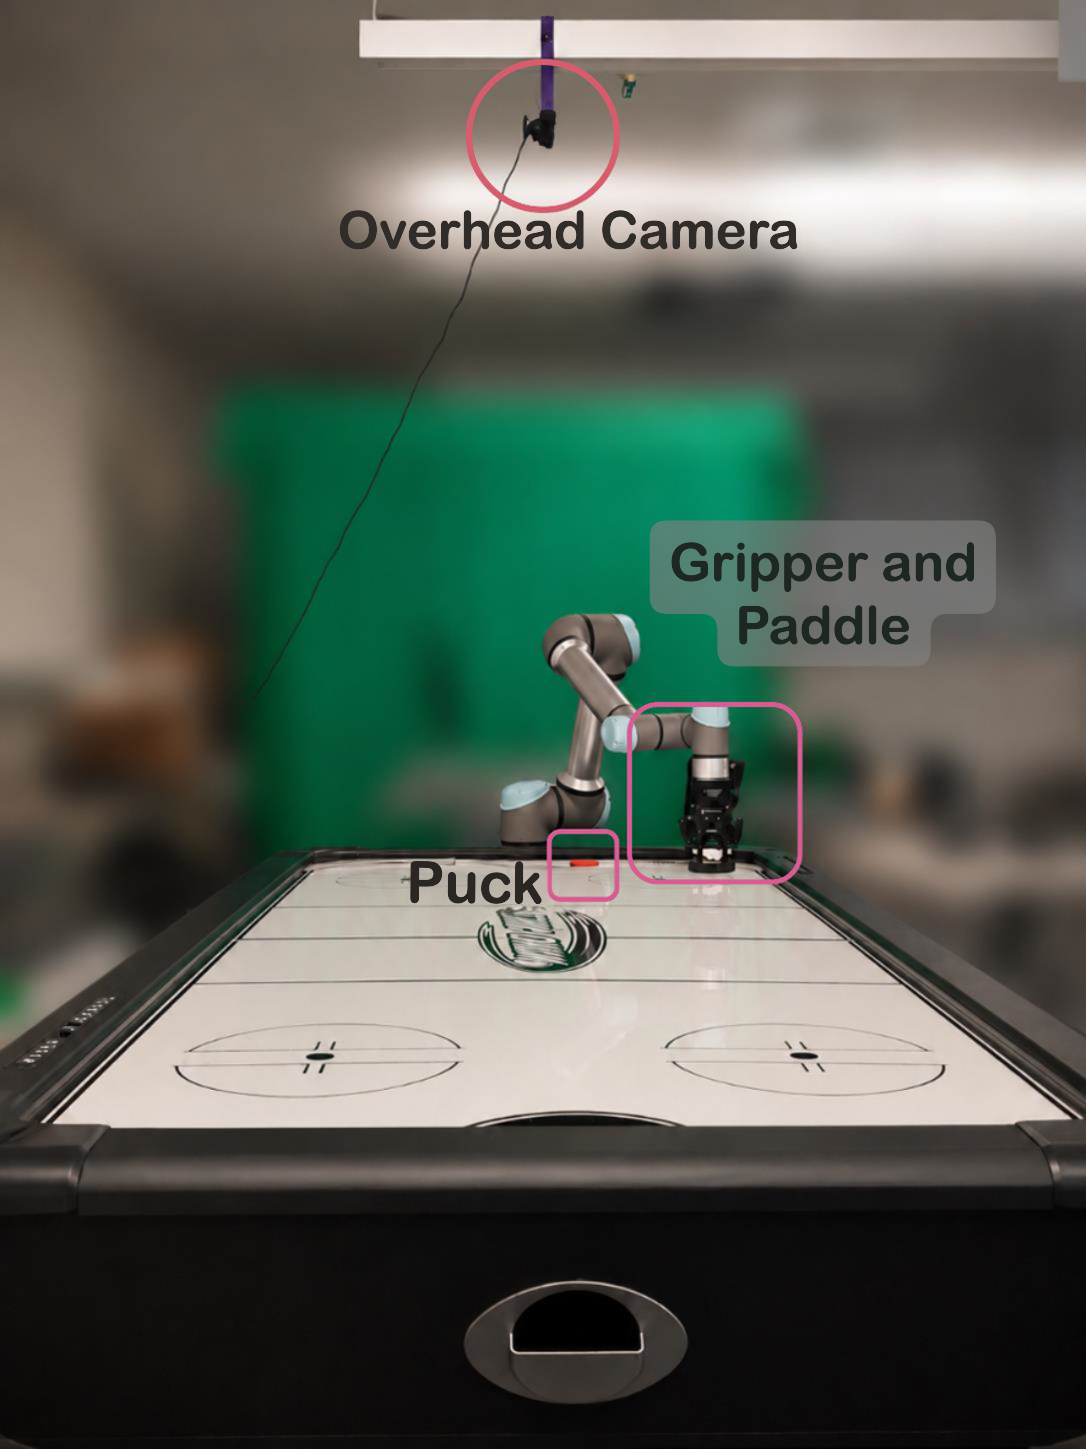
\includegraphics[width=\linewidth]{figure/air_hockey_setup.png}
%         \caption{Real-world robotic air hockey testbed.}
%         \label{fig:real_world_air_hockey_setup}
%     \end{minipage}
%     \vspace{-1em}
% \end{figure}
% All environments are wrapped as goal-conditioned vector environments.  Each
% wrapper exposes a state vector $s_t$, achieved goal $g_t^{\mathrm{ach}}$,
% desired goal $g_t^{\mathrm{des}}$, action $a_t$, and boolean success flag.  CRL
% methods use future achieved goals for contrastive relabeling; sparse-reward
% baselines use the same success flag as reward.  Episodes are automatically
% reset in the vectorized training environment.

% \begin{table}[h]
% \centering
% \small
% \setlength{\tabcolsep}{5pt}
% \caption{Backend-level simulation settings.}
% \label{tab:appendix-backend-simulation}
% \begin{tabular}{p{0.24\linewidth}p{0.18\linewidth}p{0.22\linewidth}p{0.24\linewidth}}
% \toprule
% Backend & Train horizon & Termination on success & Vectorization \\
% \midrule
% Air Hockey & $300$ steps & yes & $256$ train envs \\
% Box2D & $400$ steps in paper launch & no & $256$ train envs \\
% MetaWorld & $150$ steps & yes & async, $256$ train envs \\
% \bottomrule
% \end{tabular}
% \end{table}

% \subsection{Air Hockey}

% All paper-core Air Hockey tasks use
% \texttt{AirHockeyPuckGoalPosition-v0}.  The goal is the puck position only; the
% ``velocity'' label in the benchmark name refers to the observation mode, not to
% a velocity goal.  The success radius is
% \[
%     r_{\mathrm{goal}} = 0.06.
% \]
% The paddle, puck, and goal are randomized at reset.  The wrapper terminates an
% episode on success during training.  For the default physics tasks, episodes
% also terminate if the puck hits the bottom or passes the paddle; out-of-bounds
% termination is disabled.  For real-transfer, out-of-bounds termination is
% enabled.

% \begin{table}[h]
% \centering
% \small
% \setlength{\tabcolsep}{5pt}
% \caption{Default Air Hockey simulator parameters.}
% \label{tab:appendix-air-hockey-default-physics}
% \begin{tabular}{ll}
% \toprule
% Parameter & Value \\
% \midrule
% Simulator & Box2D Air Hockey simulator \\
% Table length / width & $1.9304$ / $0.8636$ \\
% Render size & $360$ \\
% Paddle radius & $0.0508$ \\
% Puck radius & $0.03175$ \\
% Paddle density / damping & $2500$ / $3$ \\
% Puck density / damping & $250$ / $0.5$ \\
% Gravity & $-0.5$ \\
% Force scaling & $1000$ \\
% Max force timestep & $100$ \\
% Wall bounce scale & $0.02$ \\
% Blocks / obstacles / targets & $0/0/0$ \\
% Paddles / pucks & $1/1$ \\
% Randomized paddle spawn & true \\
% Goal radius & $0.06$ \\
% \bottomrule
% \end{tabular}
% \end{table}

% \begin{table}[h]
% \centering
% \small
% \setlength{\tabcolsep}{5pt}
% \caption{Air Hockey real-transfer physics and corruption settings.}
% \label{tab:appendix-air-hockey-real-transfer}
% \begin{tabular}{ll}
% \toprule
% Parameter & Value \\
% \midrule
% Observation type & history \\
% Domain randomization & enabled \\
% Randomized variables & paddle density, puck damping, gravity \\
% Paddle density range & $[2250,3750]$ \\
% Puck damping range & $[0.1335,0.2225]$ \\
% Gravity range & $[-0.826,-0.496]$ \\
% SysID gravity & $-0.661$ \\
% SysID puck damping & $0.178$ \\
% Paddle damping & $17$ \\
% Force scaling & $0.99$ \\
% Max force timestep & $10000$ \\
% Puck density & $3000$ \\
% Paddle / puck radius & $0.0508$ / $0.03175$ \\
% Paddle restitution & $1.0$ \\
% Side / end wall restitution & $0.99$ / $0.7$ \\
% PID control & enabled \\
% PID gains & $k_p=9000$, $k_d=50$, $k_i=0$ \\
% History length & $2$ \\
% Puck observation noise & enabled, std. $0.01$ \\
% Random occlusion & enabled, start rate $0.05$ per step \\
% Occlusion length weights & $[75,39,18,9,4,2,1]$ \\
% Observation delay & enabled, $0.025$s \\
% Action delay & disabled \\
% Near-paddle puck spawn probability & $0.15$ \\
% Near-paddle spawn offset & $[0.025,0.05]$ m \\
% Near-paddle spawn speed & $[0.0,0.2]$ m/s \\
% Linear top spawn speed & $[0.0,0.5]$ m/s \\
% \bottomrule
% \end{tabular}
% \end{table}

% \subsection{Box2D}

% Box2D tasks are provided through the local \texttt{ac\_infer} checkout.  The
% paper launch uses fixed limits, reward aggregation \texttt{max}, and a horizon
% of $400$ steps for all Box2D paper-core tasks.  Success does not terminate the
% episode in the paper-core Box2D launch, which makes success-tick comparisons
% well-defined over the full horizon.

% The wrapped state is
% \[
%     s =
%     [x_c,y_c,\dot{x}_c,\dot{y}_c,\;
%       x_o,y_o,\dot{x}_o,\dot{y}_o],
% \]
% where $c$ is the controllable body and $o$ is the target/object body.  The
% achieved and desired goals are read from the underlying Box2D environment info
% dictionary.  For interaction-aware sampling, the source position is
% $(x_c,y_c)$ and the target position is $(x_o,y_o)$.

% \begin{table}[h]
% \centering
% \small
% \setlength{\tabcolsep}{5pt}
% \caption{Box2D paper-core tasks.}
% \label{tab:appendix-box2d-tasks}
% \begin{tabular}{p{0.15\linewidth}p{0.39\linewidth}p{0.34\linewidth}}
% \toprule
% Paper task name & Environment id & Variant \\
% \midrule
% Box2D center & \texttt{Box2dCenterCtrlTarget-v0} & \texttt{center-ctrl-target} \\
% Box2D goal & \texttt{Box2dGoalCtrlTarget-v0} & \texttt{goal-ctrl-target} \\
% Box2D hard & \texttt{Box2dGoalCtrlTargetHard-v0} & \texttt{goal-ctrl-target-hard} \\
% Box2D hard velocity & \texttt{Box2dGoalCtrlTargetHardVel-v0} & \texttt{goal-ctrl-target-hard-vel} \\
% Box2D maze & \texttt{Box2dMazeBallEasyNavigation-v0} & \texttt{maze-ball-easy-navigation} \\
% \bottomrule
% \end{tabular}
% \end{table}

% The hard-velocity task is a local compatibility variant implemented in the
% wrapper by taking \texttt{goal-ctrl-target-hard} and setting the target initial
% velocity to $5.0$.

% \subsection{MetaWorld}

% MetaWorld tasks use compact point observations.  The state dimension is $7$:
% \[
%     s =
%     [p_{\mathrm{hand}}\in\mathbb{R}^3,\;
%       q_{\mathrm{gripper}}\in\mathbb{R},\;
%       p_{\mathrm{object}}\in\mathbb{R}^3].
% \]
% The goal vector has the same structure:
% \[
%     g =
%     [p_{\mathrm{goal-hand}},\; q_{\mathrm{goal-gripper}},\;
%       p_{\mathrm{goal-object}}],
% \]
% with default goal gripper opening $0.4$ and default hand offset
% $(0,0,0.03)$ unless overridden by the task.  The default minimum distance
% between the initial object and sampled goal is $0.15$.  Episodes terminate on
% success during training.  The vectorized training environment uses Gymnasium
% \texttt{AsyncVectorEnv}; video rendering, when requested, uses a single-process
% render path to avoid offscreen MuJoCo context instability.

% \begin{table}[h]
% \centering
% \small
% \setlength{\tabcolsep}{5pt}
% \caption{MetaWorld paper-core tasks and success definitions.}
% \label{tab:appendix-metaworld-tasks}
% \begin{tabular}{p{0.23\linewidth}p{0.23\linewidth}p{0.22\linewidth}p{0.26\linewidth}}
% \toprule
% Paper task name & Env id & Achieved object & Success condition \\
% \midrule
% MetaWorld push & \texttt{push-v2} & object position & distance $<0.05$ \\
% MetaWorld pick place & \texttt{pick-place-v2} & object position & distance $<0.07$ \\
% MetaWorld peg insert & \texttt{peg-insert-side-v2} & peg head position & scaled distance $<0.07$ \\
% MetaWorld sweep into & \texttt{sweep-into-v2} & object position & distance $<0.05$ and $z$ error $<0.02$ \\
% \bottomrule
% \end{tabular}
% \end{table}

% The \texttt{peg-insert-side-v2} wrapper maps to the canonical
% \texttt{peg-insert-side-v3} task, uses success scale $(1,2,2)$, and uses a
% goal hand offset $(0.13,0,0.03)$.  The \texttt{sweep-into-v2} success
% calculation ignores the target $z$ axis for the main distance while enforcing a
% separate $z$-axis threshold of $0.02$.

% \subsection{Post-Hoc Air Hockey Consecutive Evaluation}

% For the one-minute Air Hockey challenge, evaluation is separate from training.
% The evaluator disables terminate-on-success so the puck can be re-armed to a
% new goal after each success.  The standard setting is
% \[
%     \text{horizon}=1200\text{ steps},\qquad
%     \text{seeds}=1,\ldots,16.
% \]
% The recorded metrics are complete rate, mean number of consecutive goals, and
% maximum number of consecutive goals.  Rendering is disabled by default for
% batch evaluation, but the same evaluator can render rollout videos for selected
% checkpoints.

% \subsection{Reproducibility Pointers}

% The benchmark gallery is defined by
% \texttt{benchmark/configs/envs/}.  The paper-core suite composition is defined
% by \texttt{benchmark/testbed/suites/paper\_core.yaml}.  The generated concrete
% launch commands are stored under \texttt{benchmark/testbed/tasks/paper\_core/}.
% The Air Hockey physical parameters above are copied from
% \texttt{src/unsupervised\_manipulation/envs/air\_hockey\_configs/}.
